\documentclass[a4paper,twocolumn,draft=true]{scrartcl}
\usepackage{graphicx}
\usepackage{todonotes}
\title{The HICANN Floating Gate Analog Memory}
\subtitle{A measurement protocol}
\author{Andreas Hartel}

\begin{document}
\maketitle
\section{Measurement setup and signal integrity}
The first question one has to ask is: What do we measure? And how do we measure it?
We measure voltages via an FPGA-base digitizer board that gets it's input voltage via a flat ribbon cable
with a $50\Omega$ termination.
The signal path is rather long:
The signal of the floating gate cells with a voltage output (source follower) is routed to an output buffer that directly drives the $50\Omega$ output. The distance between a floating gate's source follower and the output buffer can be up to approximately 1.5 mm.
The output buffer drives a line accross the main PCB that connects to the wafer and from the main PCB via a flat ribbon cable (of approximately 0.5 m length) to the ADC board.
This type of routing can cause crosstalk.

The signal integrity can also be impaired by other Hicann chip's outputs that are connected to one another within a reticle.

12 out of 24 lines of floating gate cells in a block have a current source output.
Their output current gets converted to a voltage via a ohmic resistor of nominally $153.5 k\Omega$.
\todo[fancyline]{Measure!}This resitor's value can even be measured.

% 
% Following lines commented out because strange x-axis on plots
%
%The signal integrity is shown in figures \ref{fig:noise_voltage_cell} and \ref{fig:noise_current_cell}.
%
%\begin{figure}
%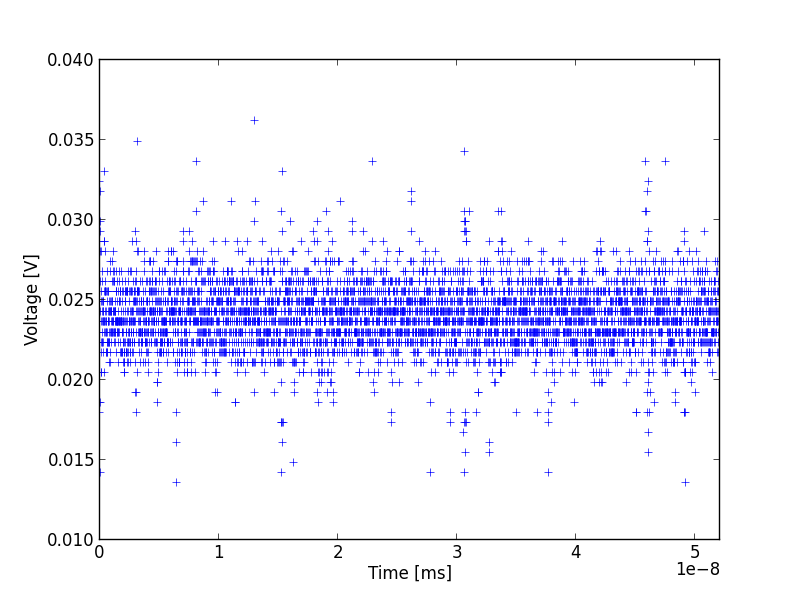
\includegraphics[scale=.34]{figures/trace_0_23_7.png}
%\caption{Voltage cell, row 0, cell 23}
%\label{fig:noise_voltage_cell}
%\end{figure}
%\begin{figure}
%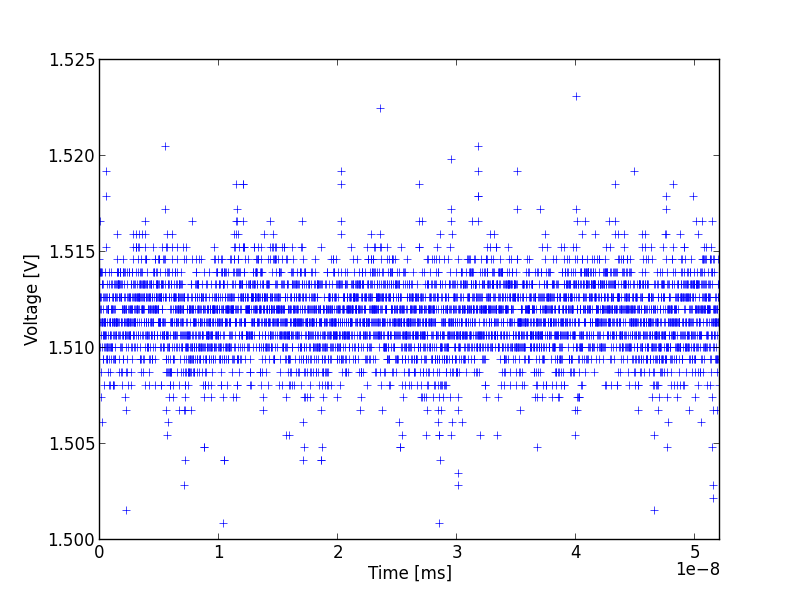
\includegraphics[scale=.34]{figures/trace_1_23_7.png}
%\caption{Current cell, row 1, cell 23}
%\label{fig:noise_current_cell}
%\end{figure}

\section{Drift}
A floating gate block was programmed to DAC value 511 once at the beginng.
Afterwards the programmed values of all cells was measured once and then
49 times more with at least 10 seconds distance between two succesive measurements.
The first and last values of all cells' measurements were subtracted and plotted in figure \ref{fig:drift_0}. 	
The plot is divided into current and voltage cells. The horizontal lines show the mean drift.
Some measurements points have been cut off to yield a better resolution on the y-axis.
It can be seen that the drift is larger for voltage cells than for current cells but is 
less than 2 mV in 49 minutes.
\begin{figure}
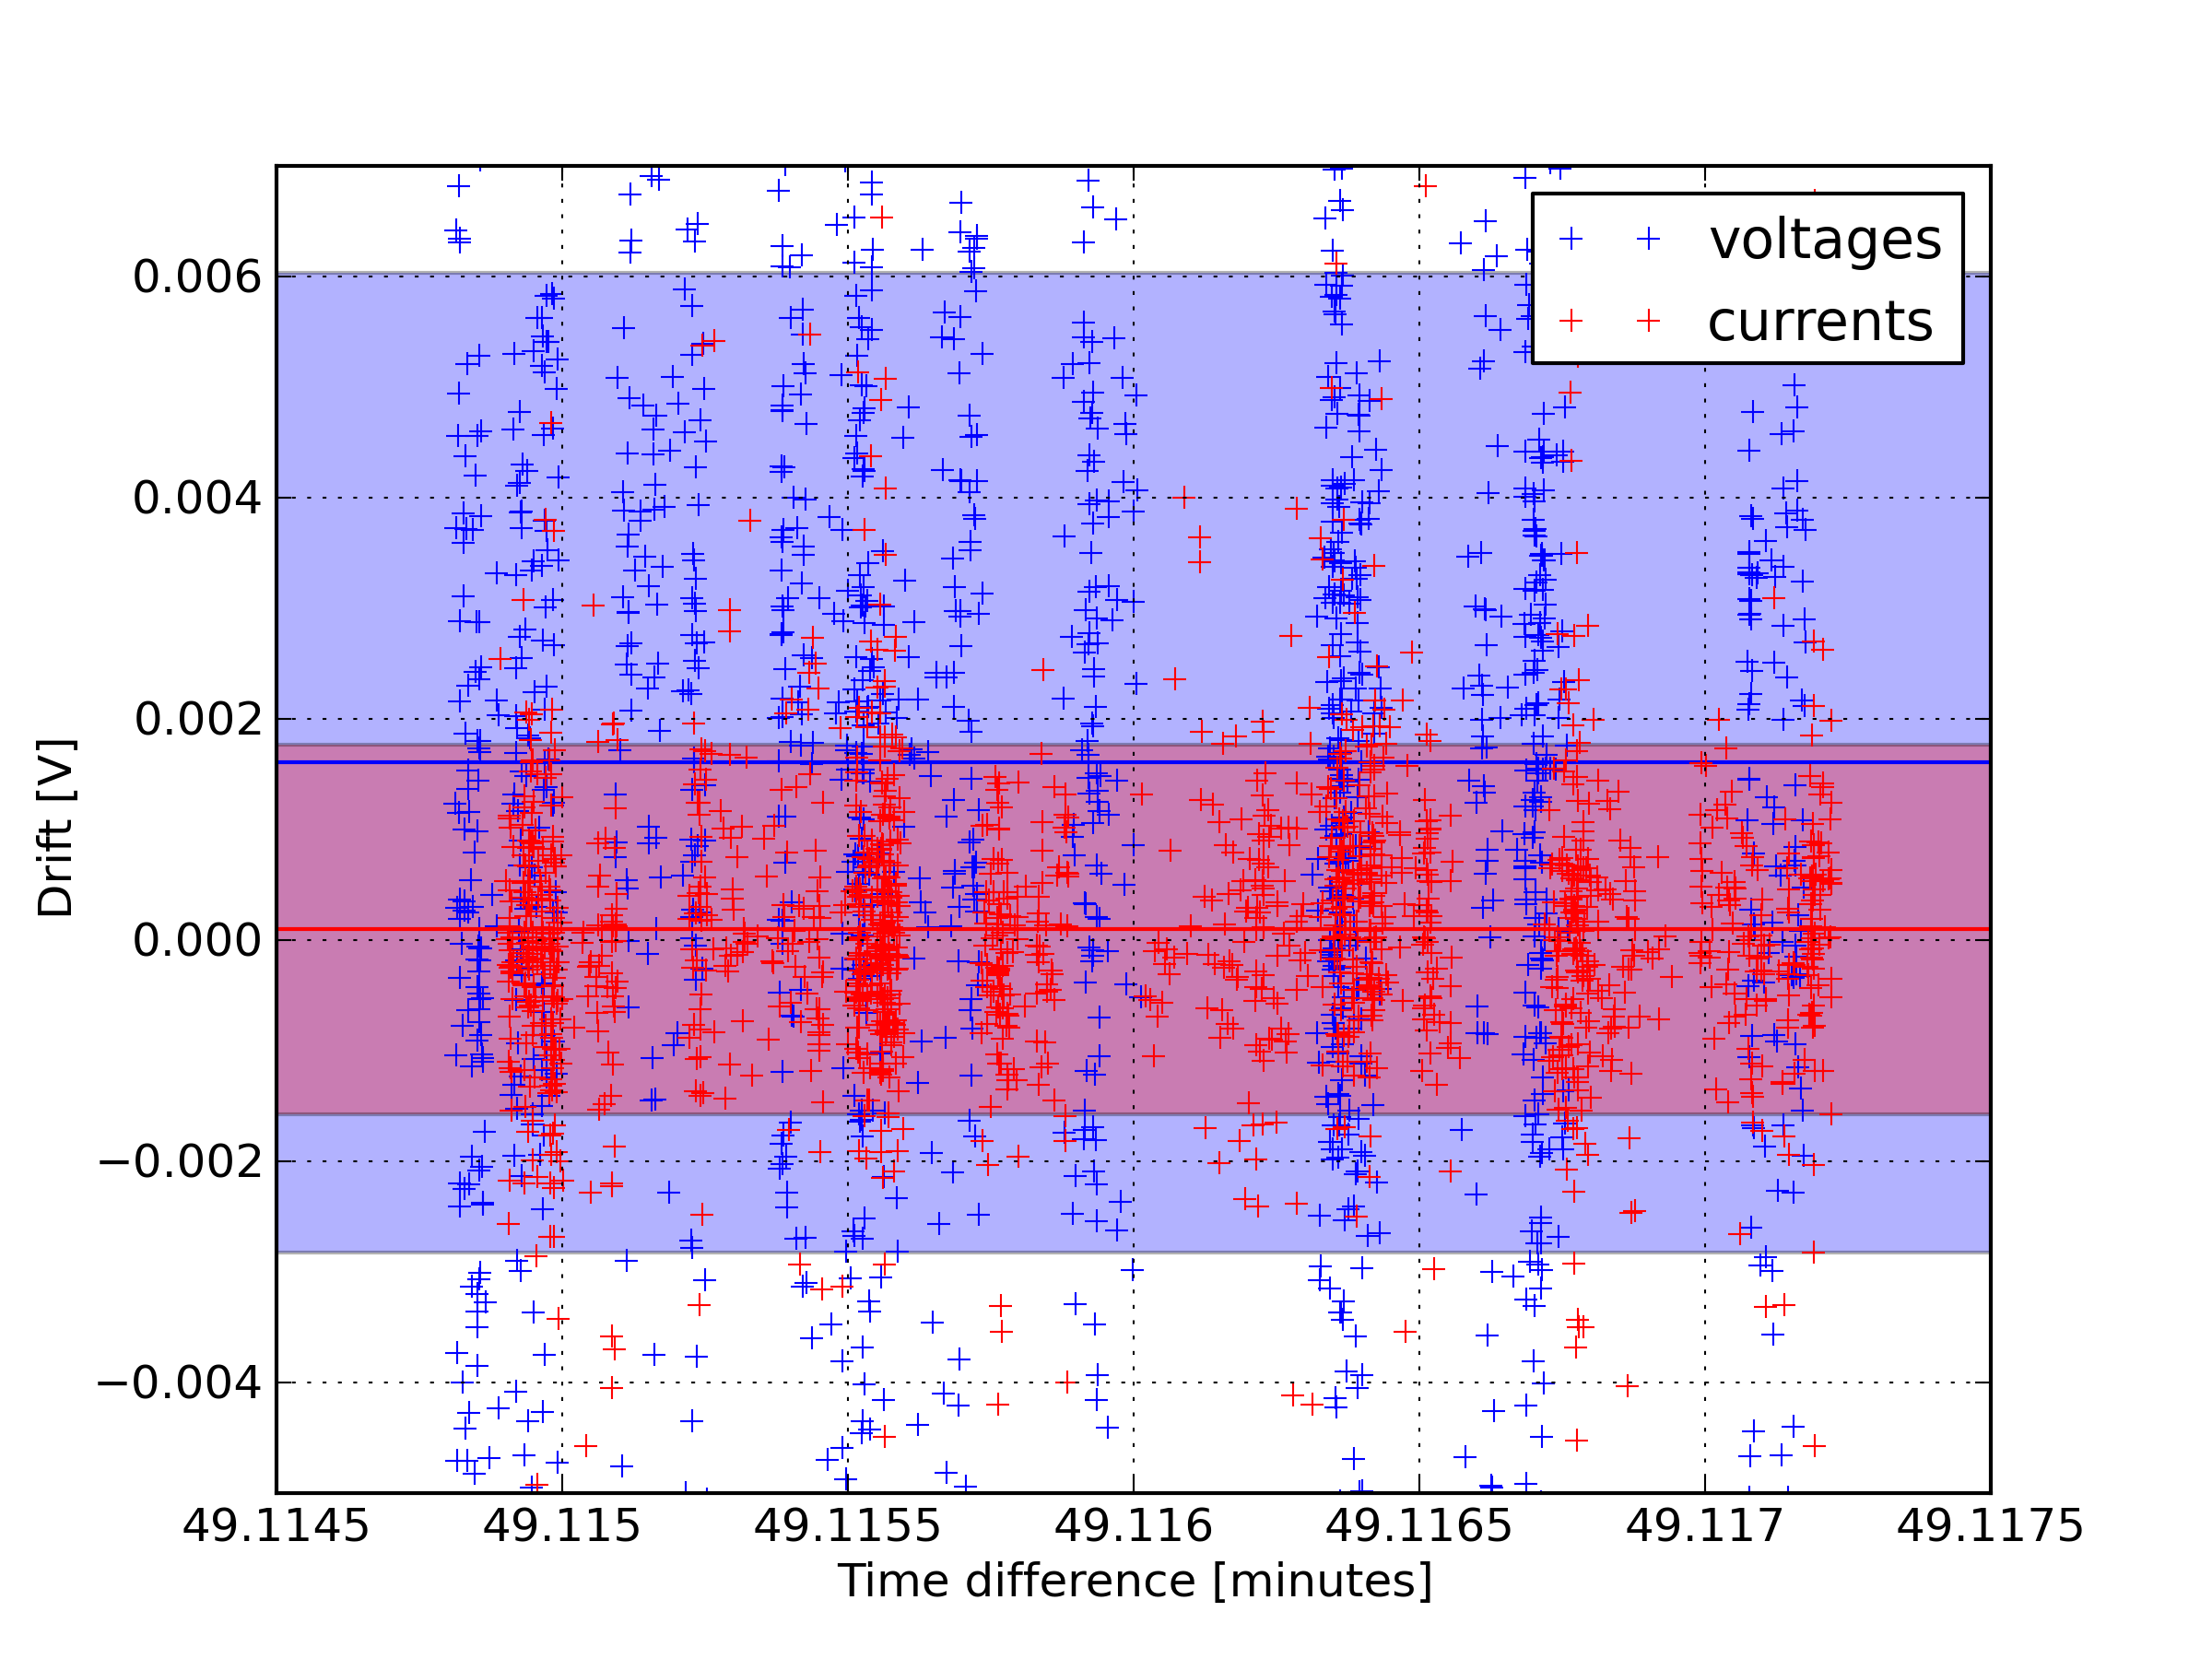
\includegraphics[scale=.34]{{figures/FG0_HC0_DNC0_FPGA192.168.1.1_511_norp_drift}.png}
\caption{Wafer 0, Reticle 21, Hicann 0, FGblock 0, Horizontal rows show mean drift, colored areas show standard deviation.}
\label{fig:drift_0}
\end{figure}

\section{Sensitivity}
A single row of a single FG block of a single Hicann is programmed to a maximum output voltage.
Subsequently, several programming pulses are applied that lower the floating gate voltage.
The impact of these equally long programming pulses is plotted depenging on the current floating gate voltage.

The floating gate cells of this row are then programmed to lowest voltage and the process is repeated with equally long pulses that raise the floating gate voltge.

Figures \ref{fig:pulse_characterization_current_15_20} and \ref{fig:pulse_characterization_voltage_15_20} show the impact of pulses of width 15 (for lowering FG voltage) and 20 (for raising FG voltage) for current and voltage cells respectively.
It can be seen, that voltage cells are less sensitive to the programming pulses.

Also, lowering the FG voltage by the same amount takes smaller programming pulses in both cases.

\begin{figure}
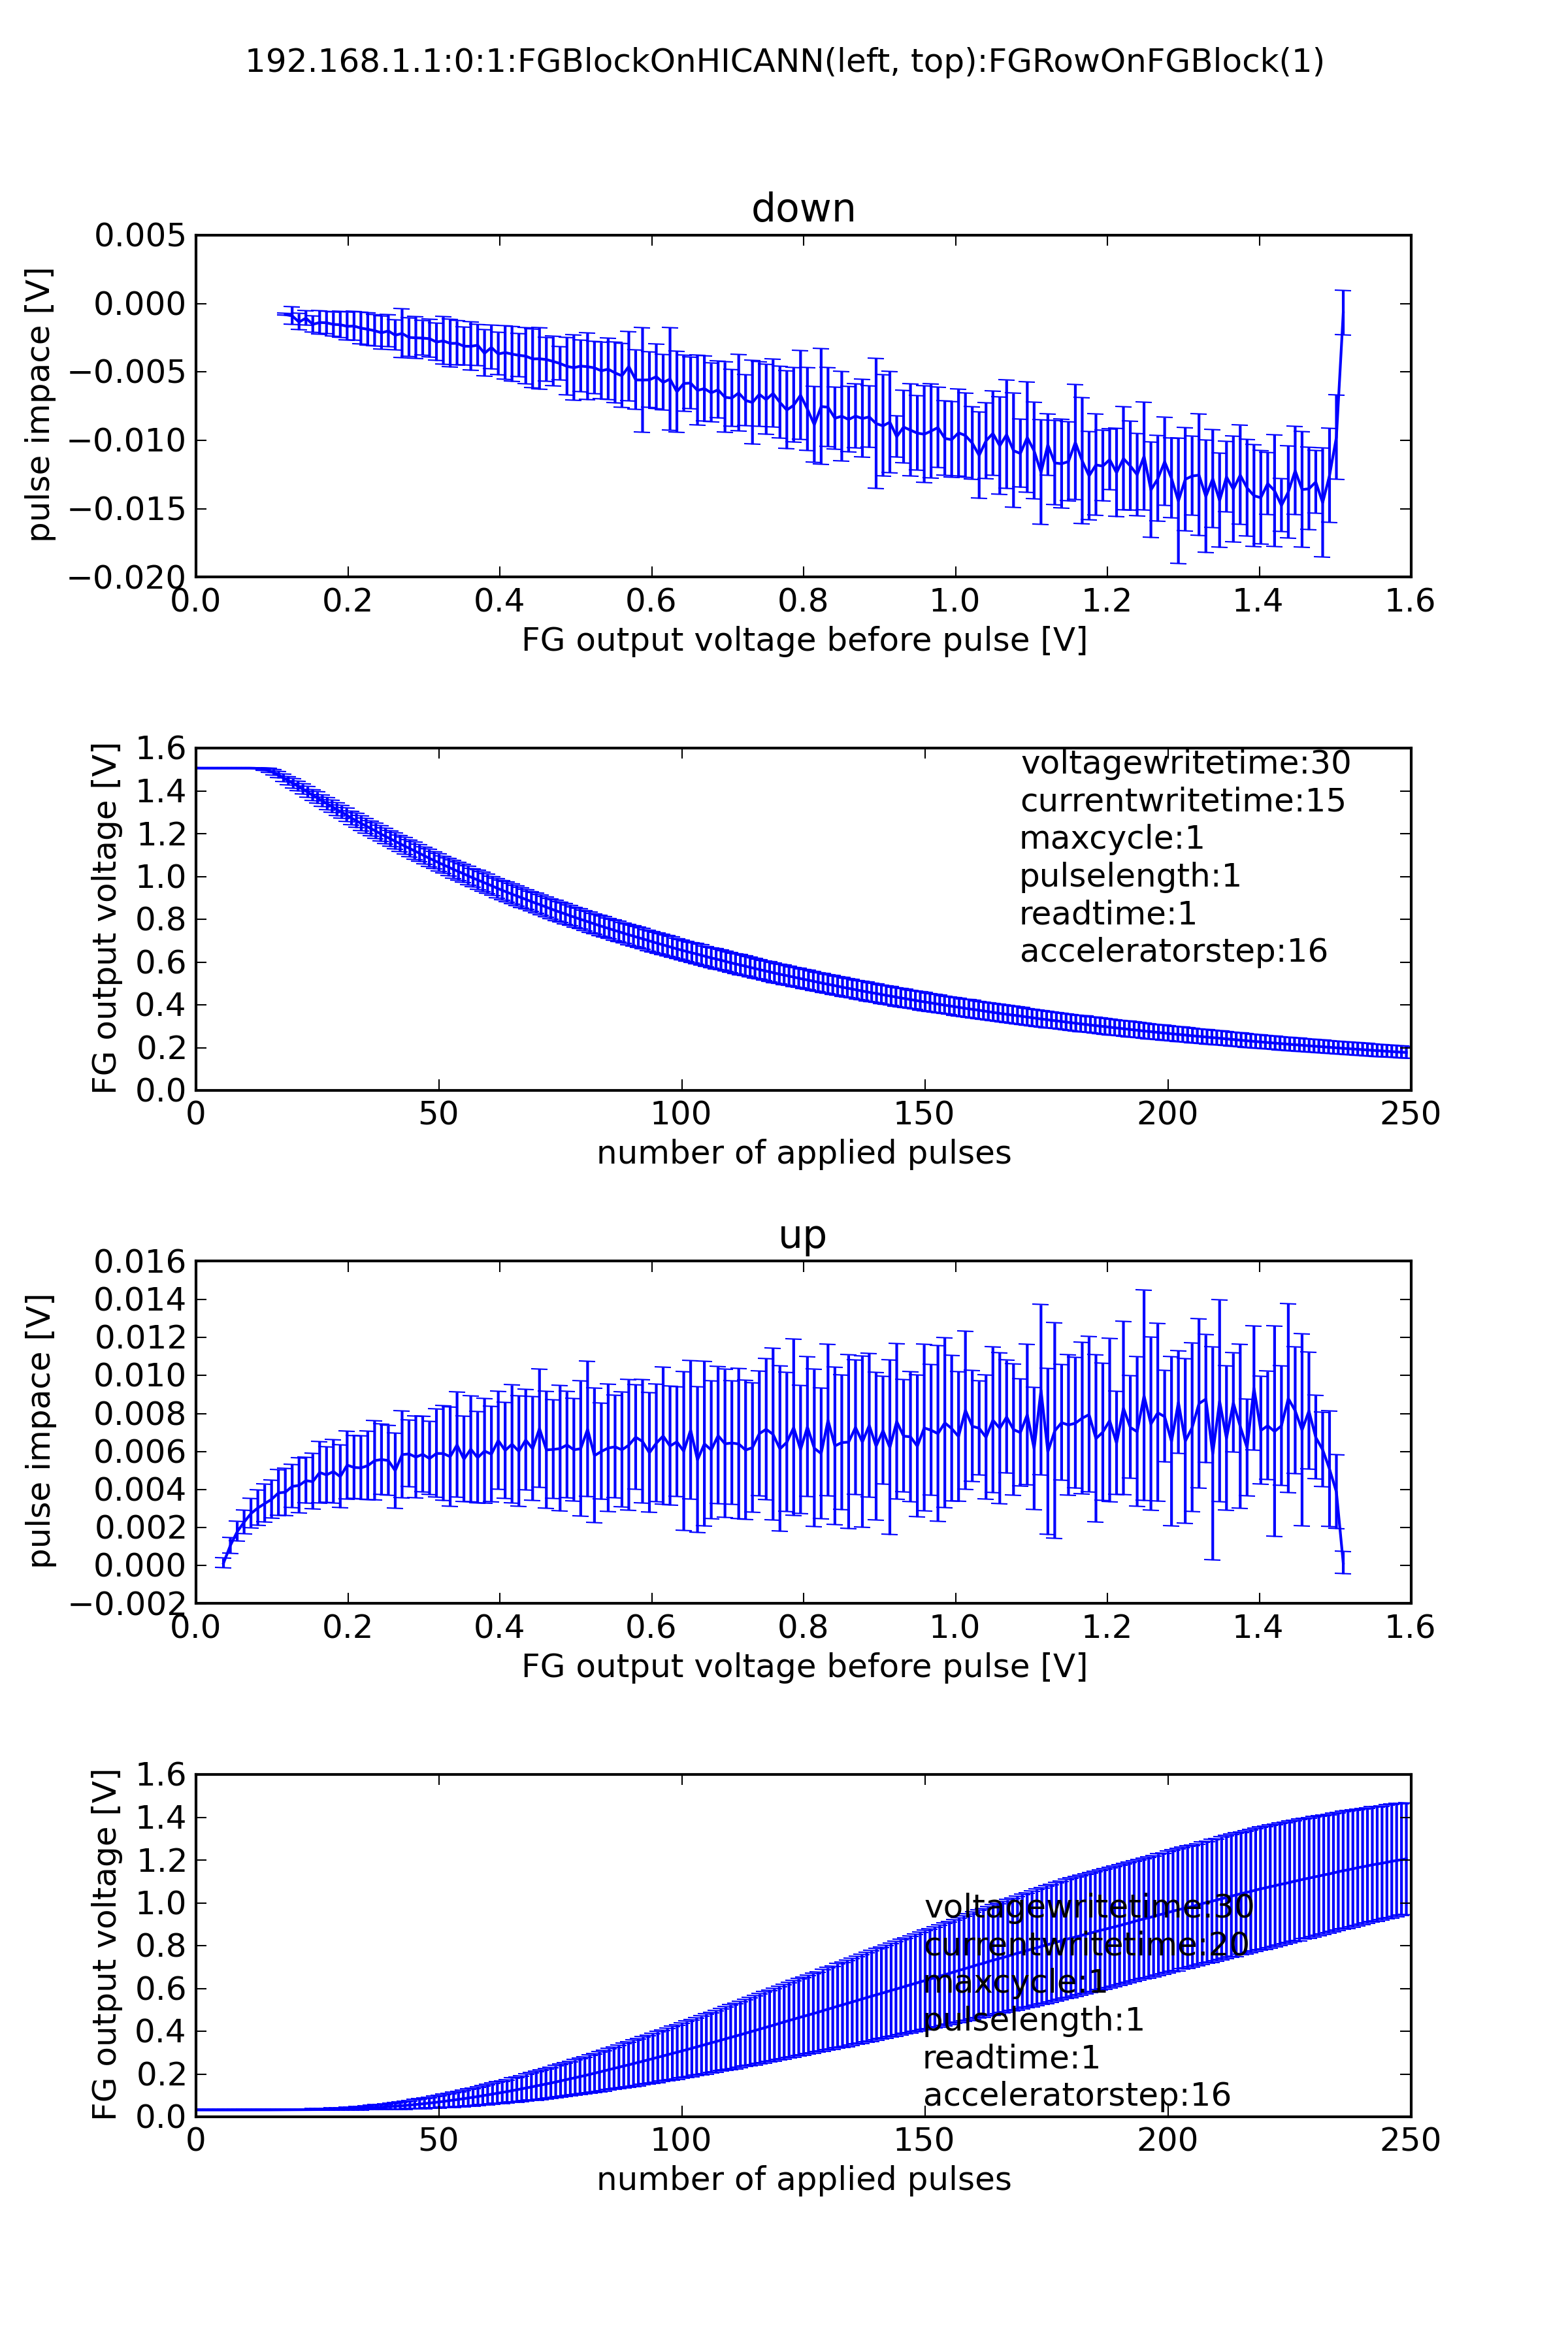
\includegraphics[scale=.35]{figures/pulse_characterization_current_15_20.png}
\caption{Impact of floating gate programming pulses on row 1 (current cells) on the top-left floating gate block on hicann 1 on Reticle 21 on Wafer 0}
\label{fig:pulse_characterization_current_15_20}
\end{figure}

\begin{figure}
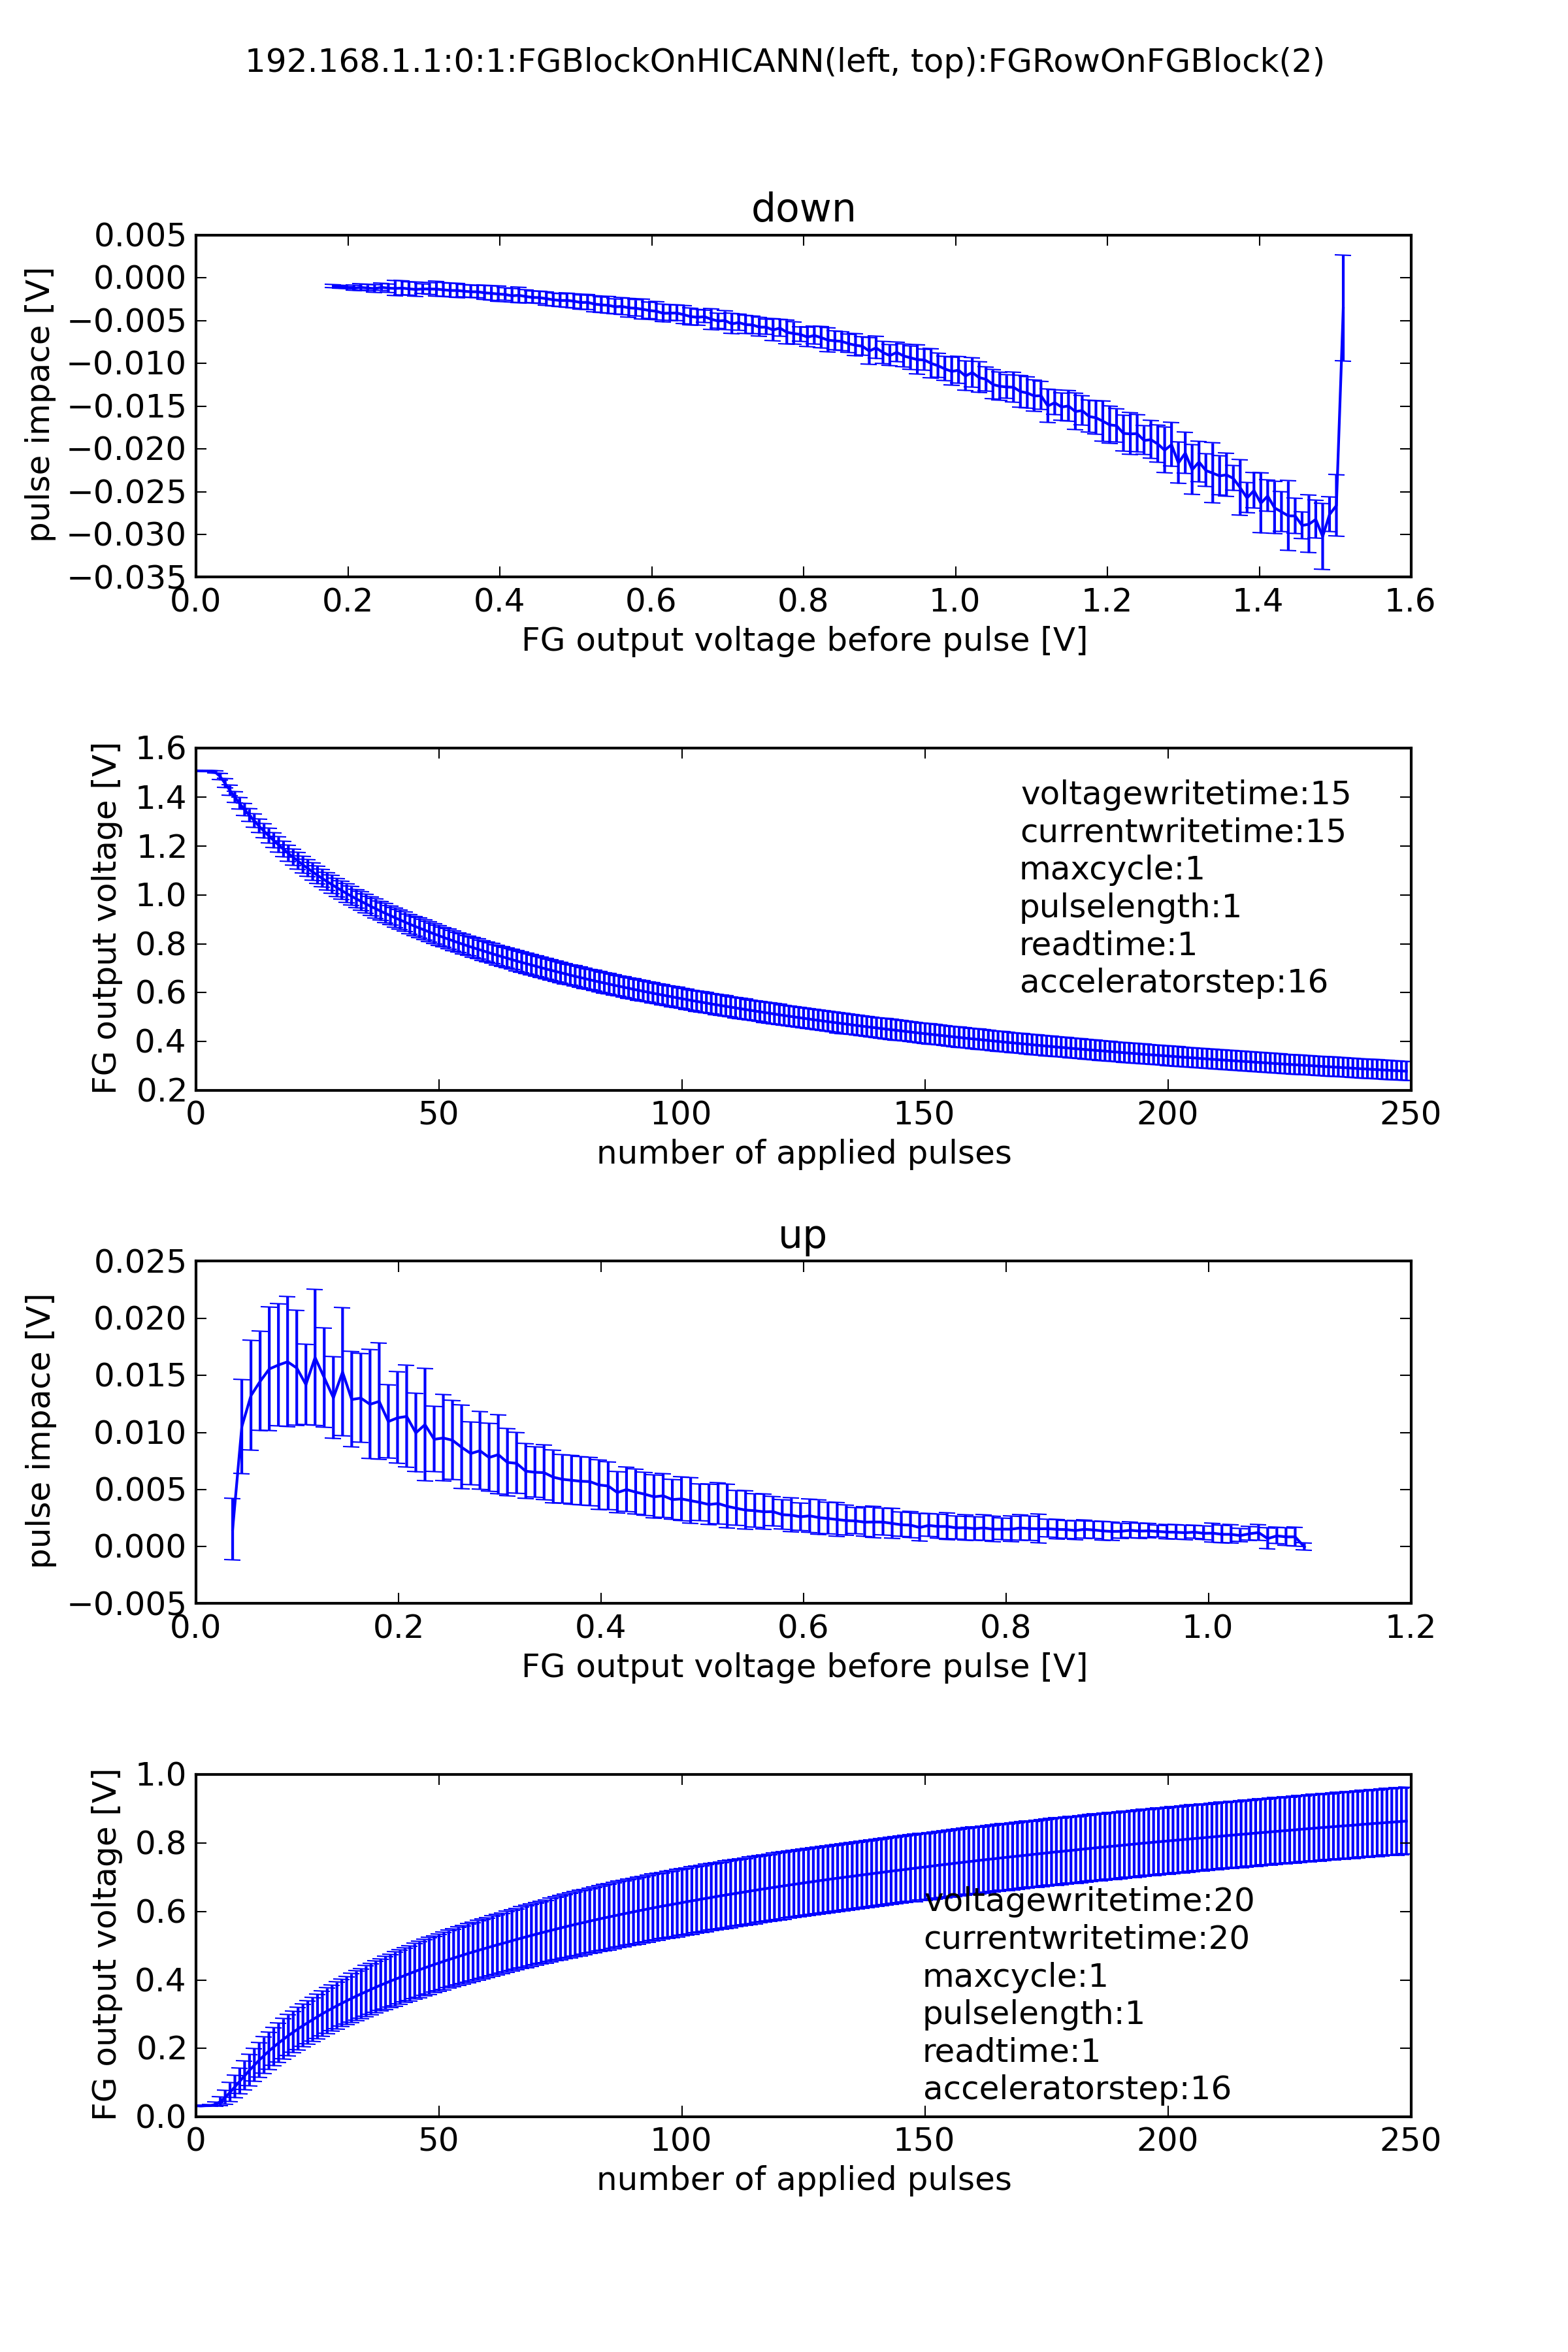
\includegraphics[scale=.35]{figures/pulse_characterization_voltage_15_20.png}
\caption{Impact of floating gate programming pulses on row 2 (voltage cells) on the top-left floating gate block on hicann 1 on Reticle 21 on Wafer 0}
\label{fig:pulse_characterization_voltage_15_20}
\end{figure}

\section{Repeatability}
When programming a single row of a single FG block of a single Hicann repeatedly with random values for each cell one gets an estimate of the reproducability of the different target values.
A resulting measurement for the programming parameters and the programming scheme used as of commit 1d15fd50 can be found in figure \ref{fig:row_progrow_default_current} for current cells and in figure \ref{fig:row_progrow_default_voltage} for voltage cells.
The green line in these plots shows the average of the standard deviation for DAC values between 0 and 800.
The programming parameters are listed in \ref{tab:default_fg_values}.

\begin{figure}
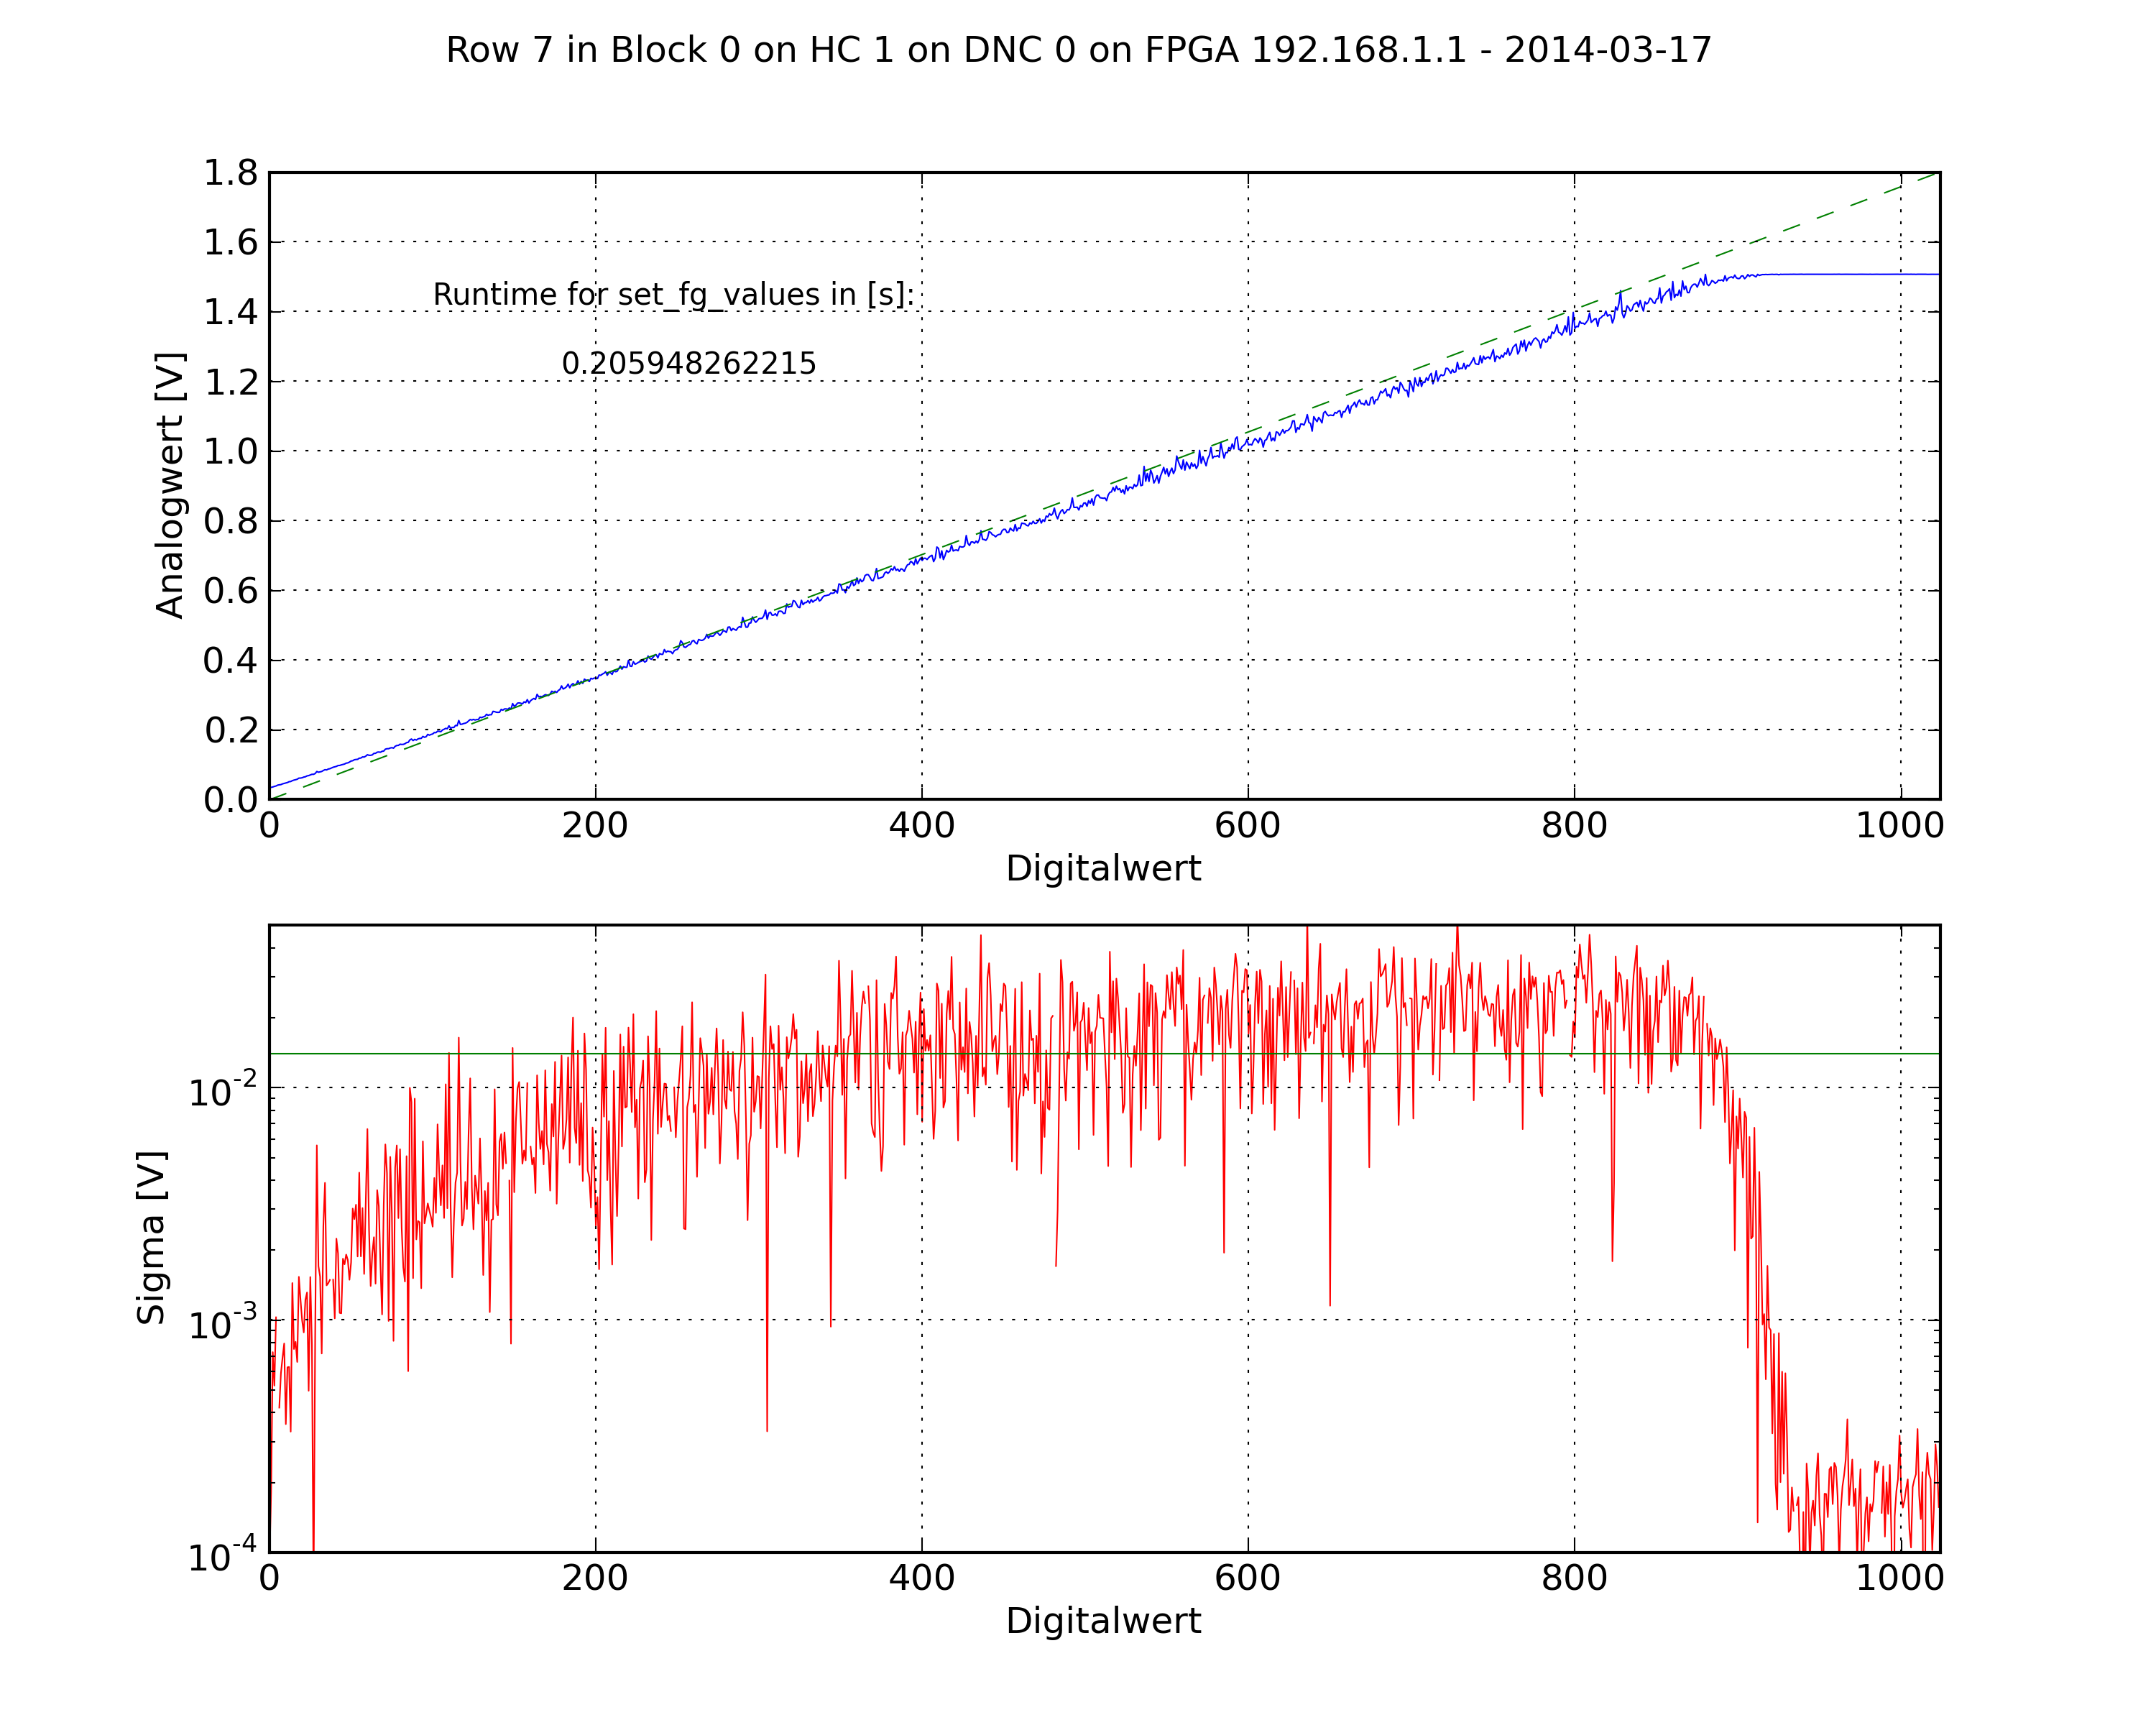
\includegraphics[scale=.28]{figures/single_row_random_progonerow_default_current.png}
\caption{Current cells: 50 repeated runs of programming one single row to random values and reading out all cells of the row with the ADC board. Plotted are the mean values for every digital target value in the upper plot and the standard deviation in the lower plot.}
\label{fig:row_progrow_default_current}
\end{figure}

\begin{figure}
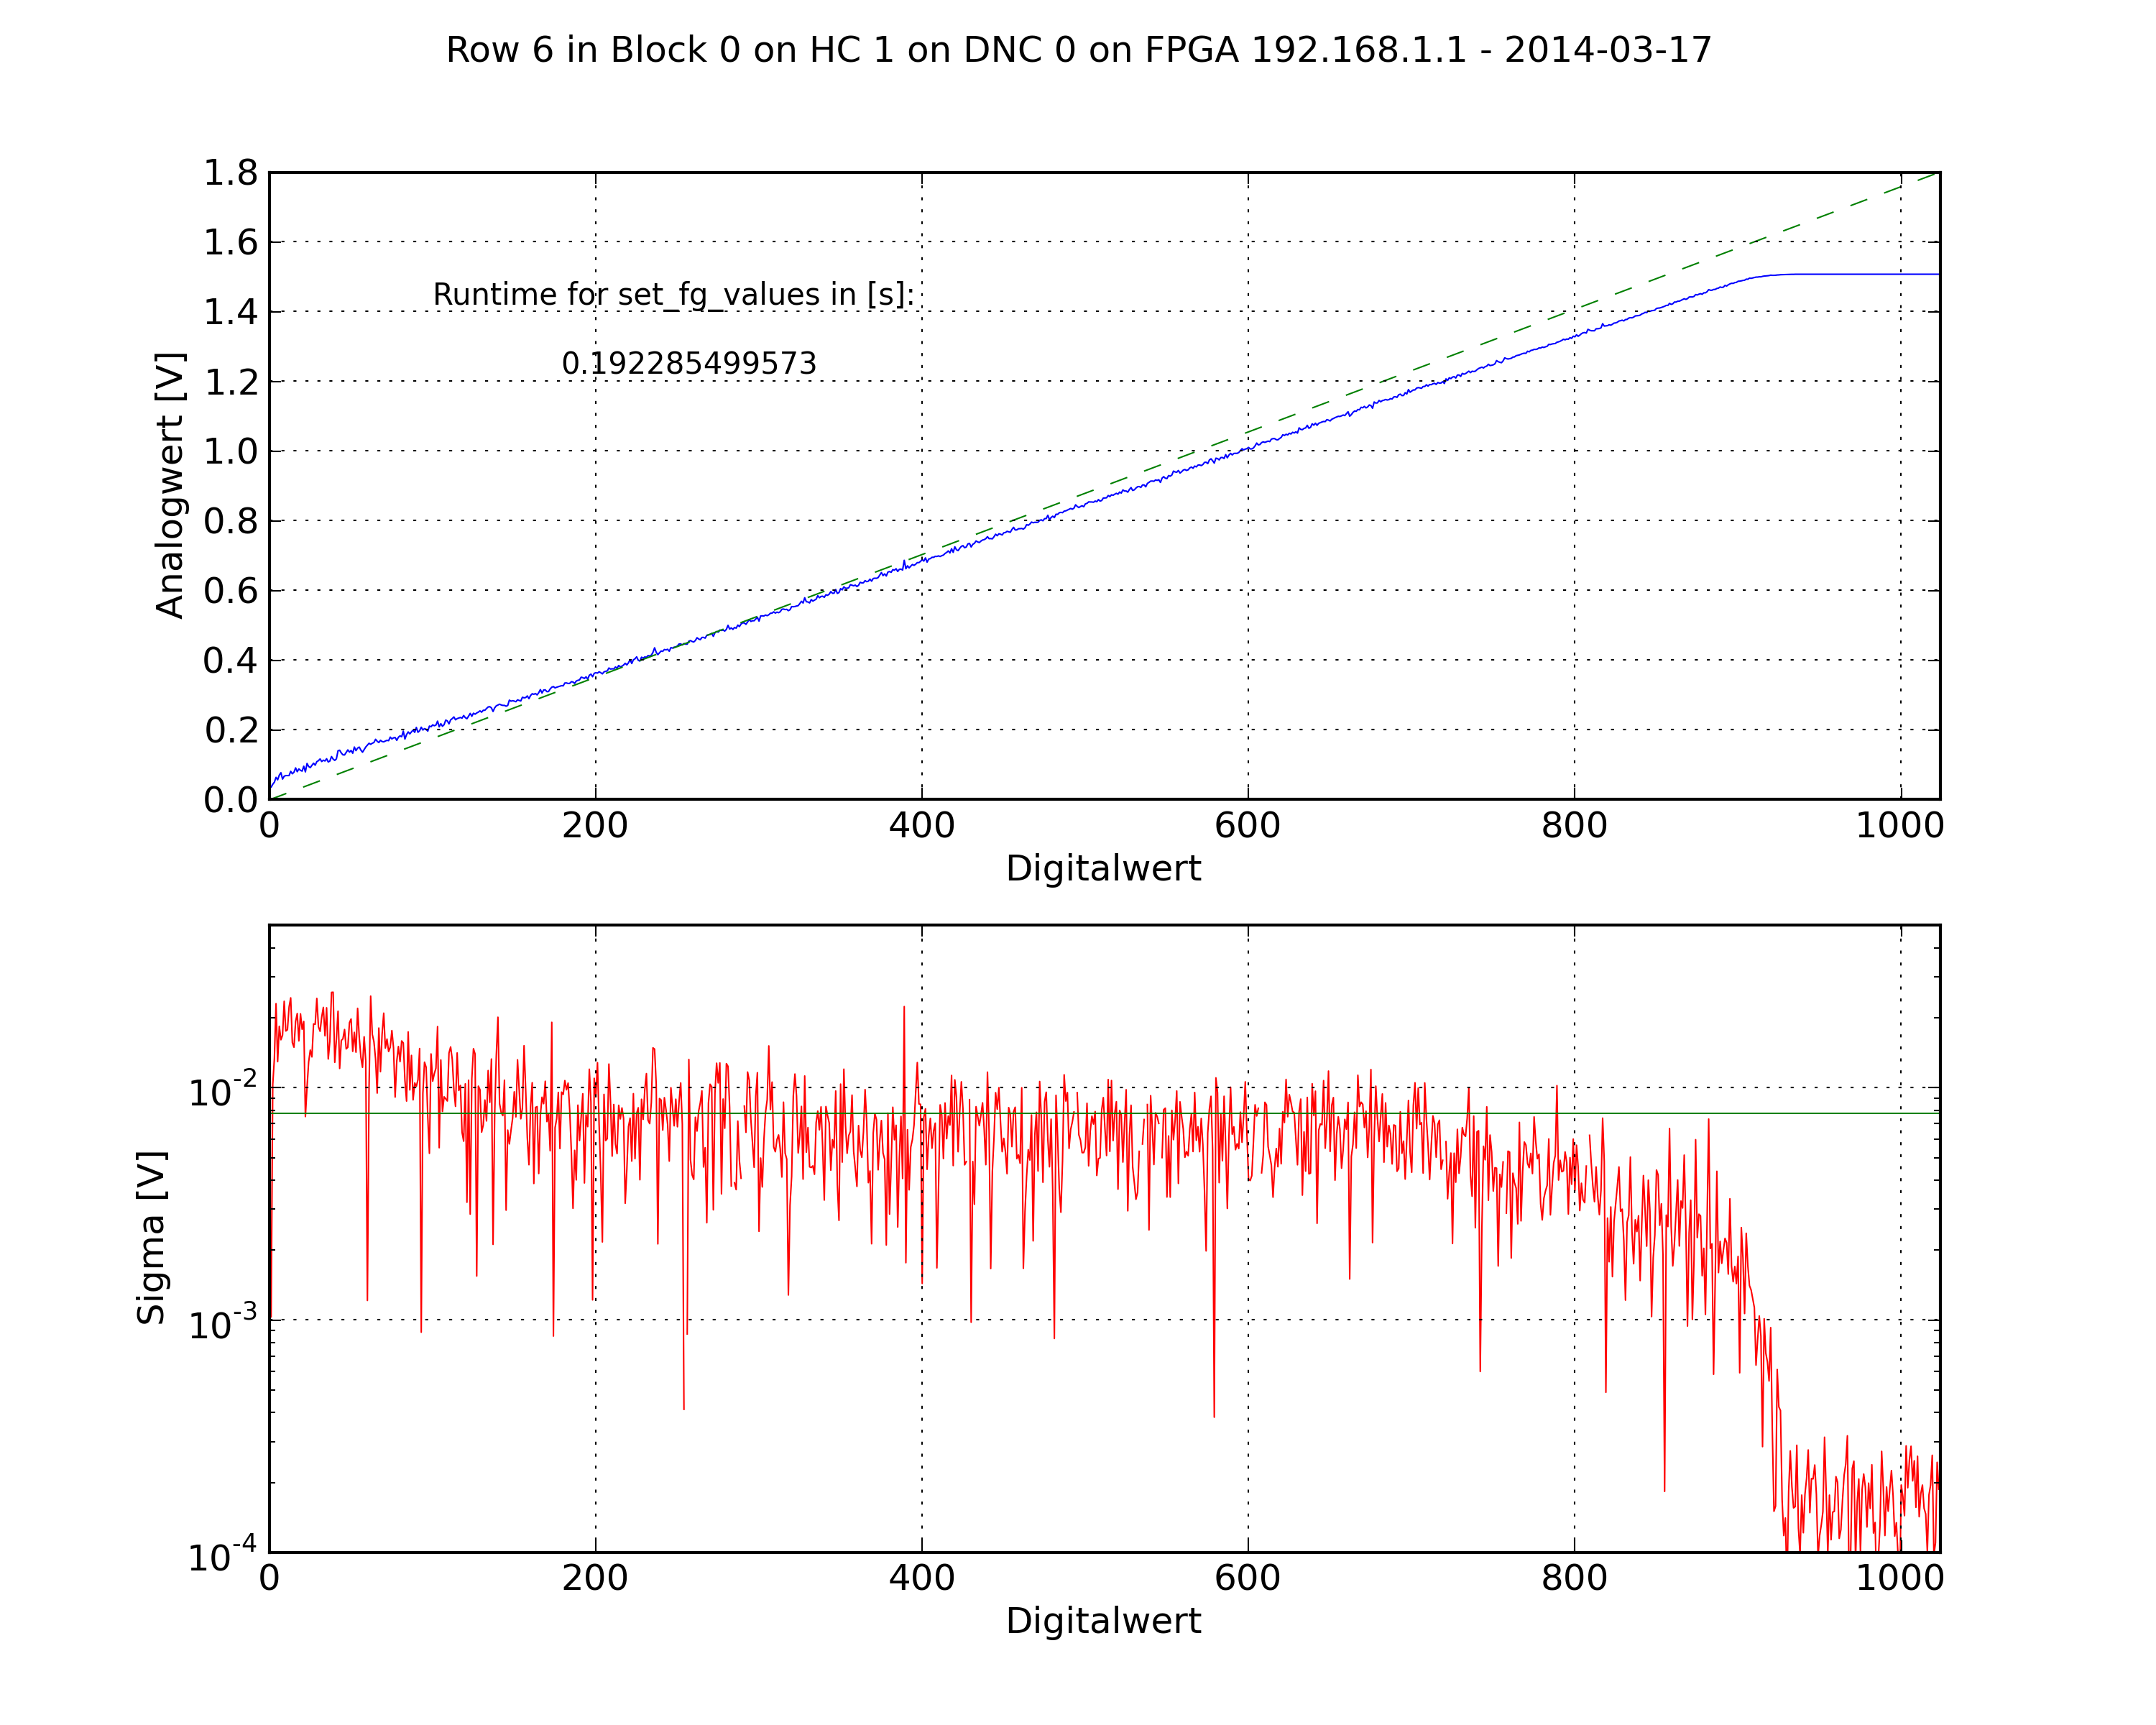
\includegraphics[scale=.28]{figures/single_row_random_progonerow_default_voltage.png}
\caption{Voltage cells: 50 repeated runs of programming one single row to random values and reading out all cells of the row with the ADC board. Plotted are the mean values for every digital target value in the upper plot and the standard deviation in the lower plot.}
\label{fig:row_progrow_default_voltage}
\end{figure}

To improve the precision of the floating gate programming process, a second programming cycle has been introduced.
The programming parameters for the second programming cycle are listed in table \ref{tab:afterburn_fg_values}.
The resulting precision for the random value test in a single row can be seen in figures \ref{fig:row_progrow_default_voltage} and \ref{fig:row_progrow_default_current}.

\begin{figure}
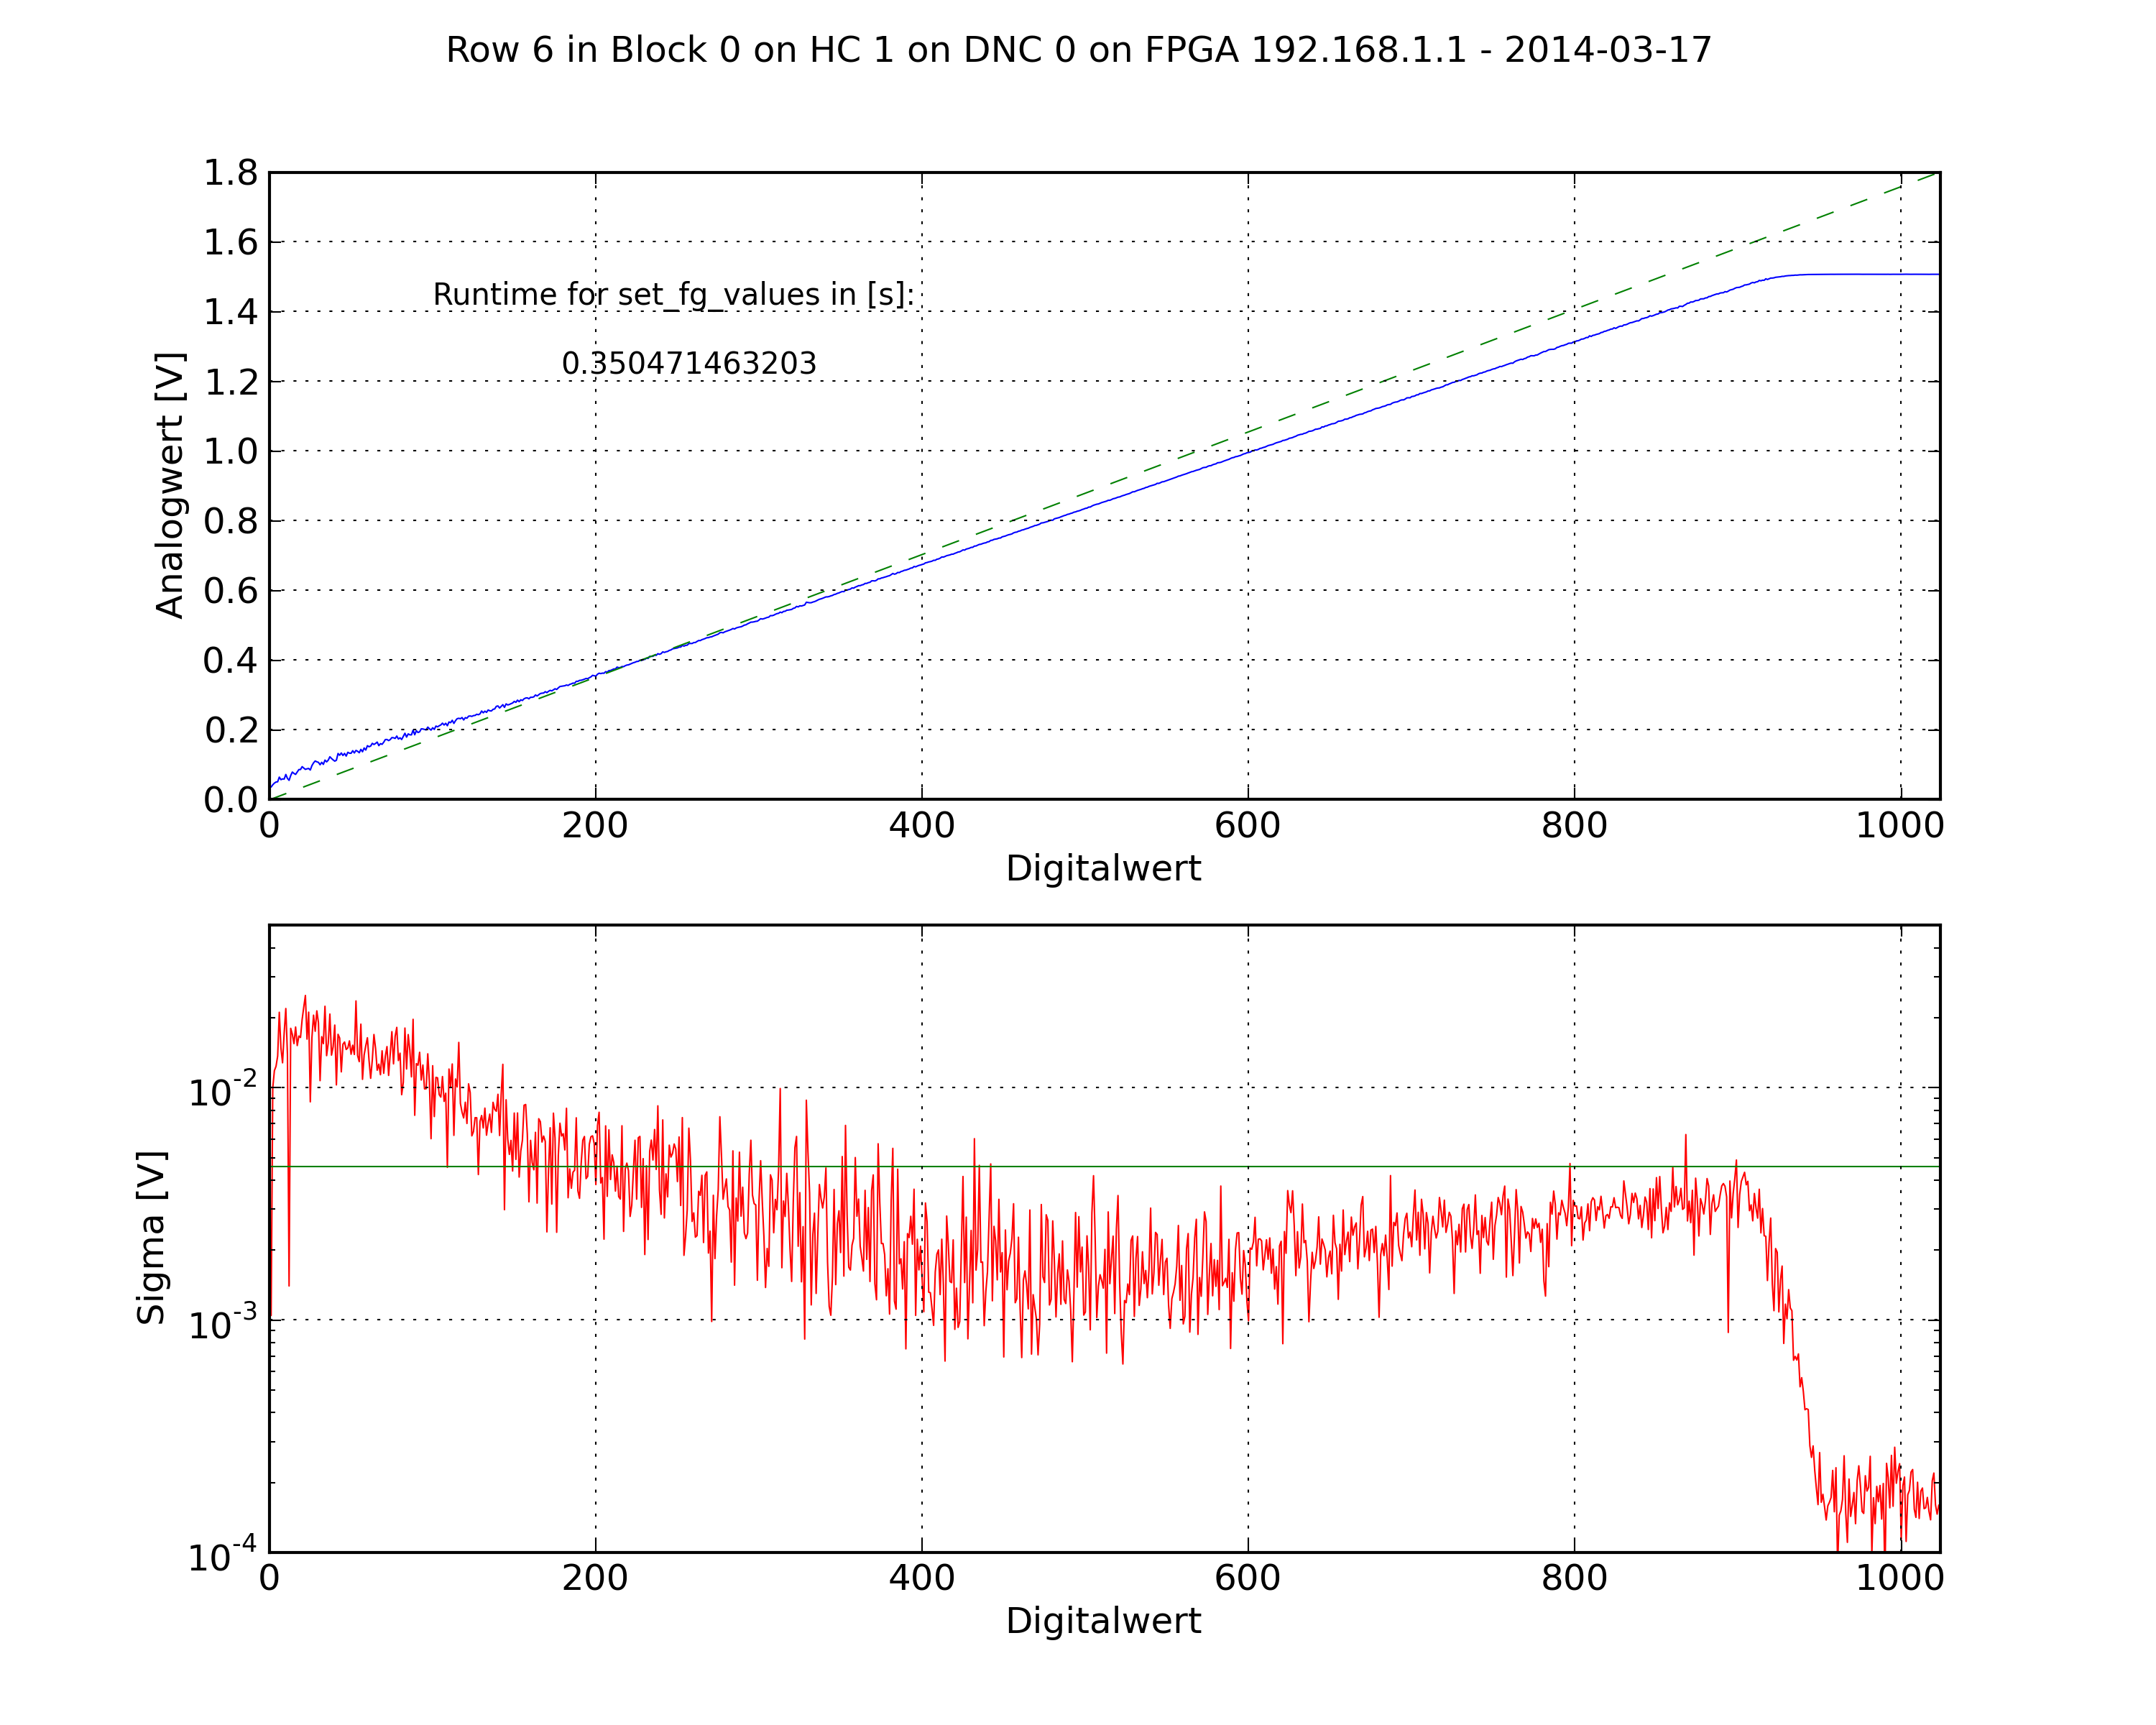
\includegraphics[scale=.28]{figures/single_row_random_progonerow_afterburn_voltage.png}
\caption{Voltage cells: 100 repeated runs of programming one single row to random values and reading out all cells of the row with the ADC board. The programming is done in two steps, once with default programming parameters and afterwards with short pulses.}
\label{fig:row_progrow_default_voltage}
\end{figure}

\begin{figure}
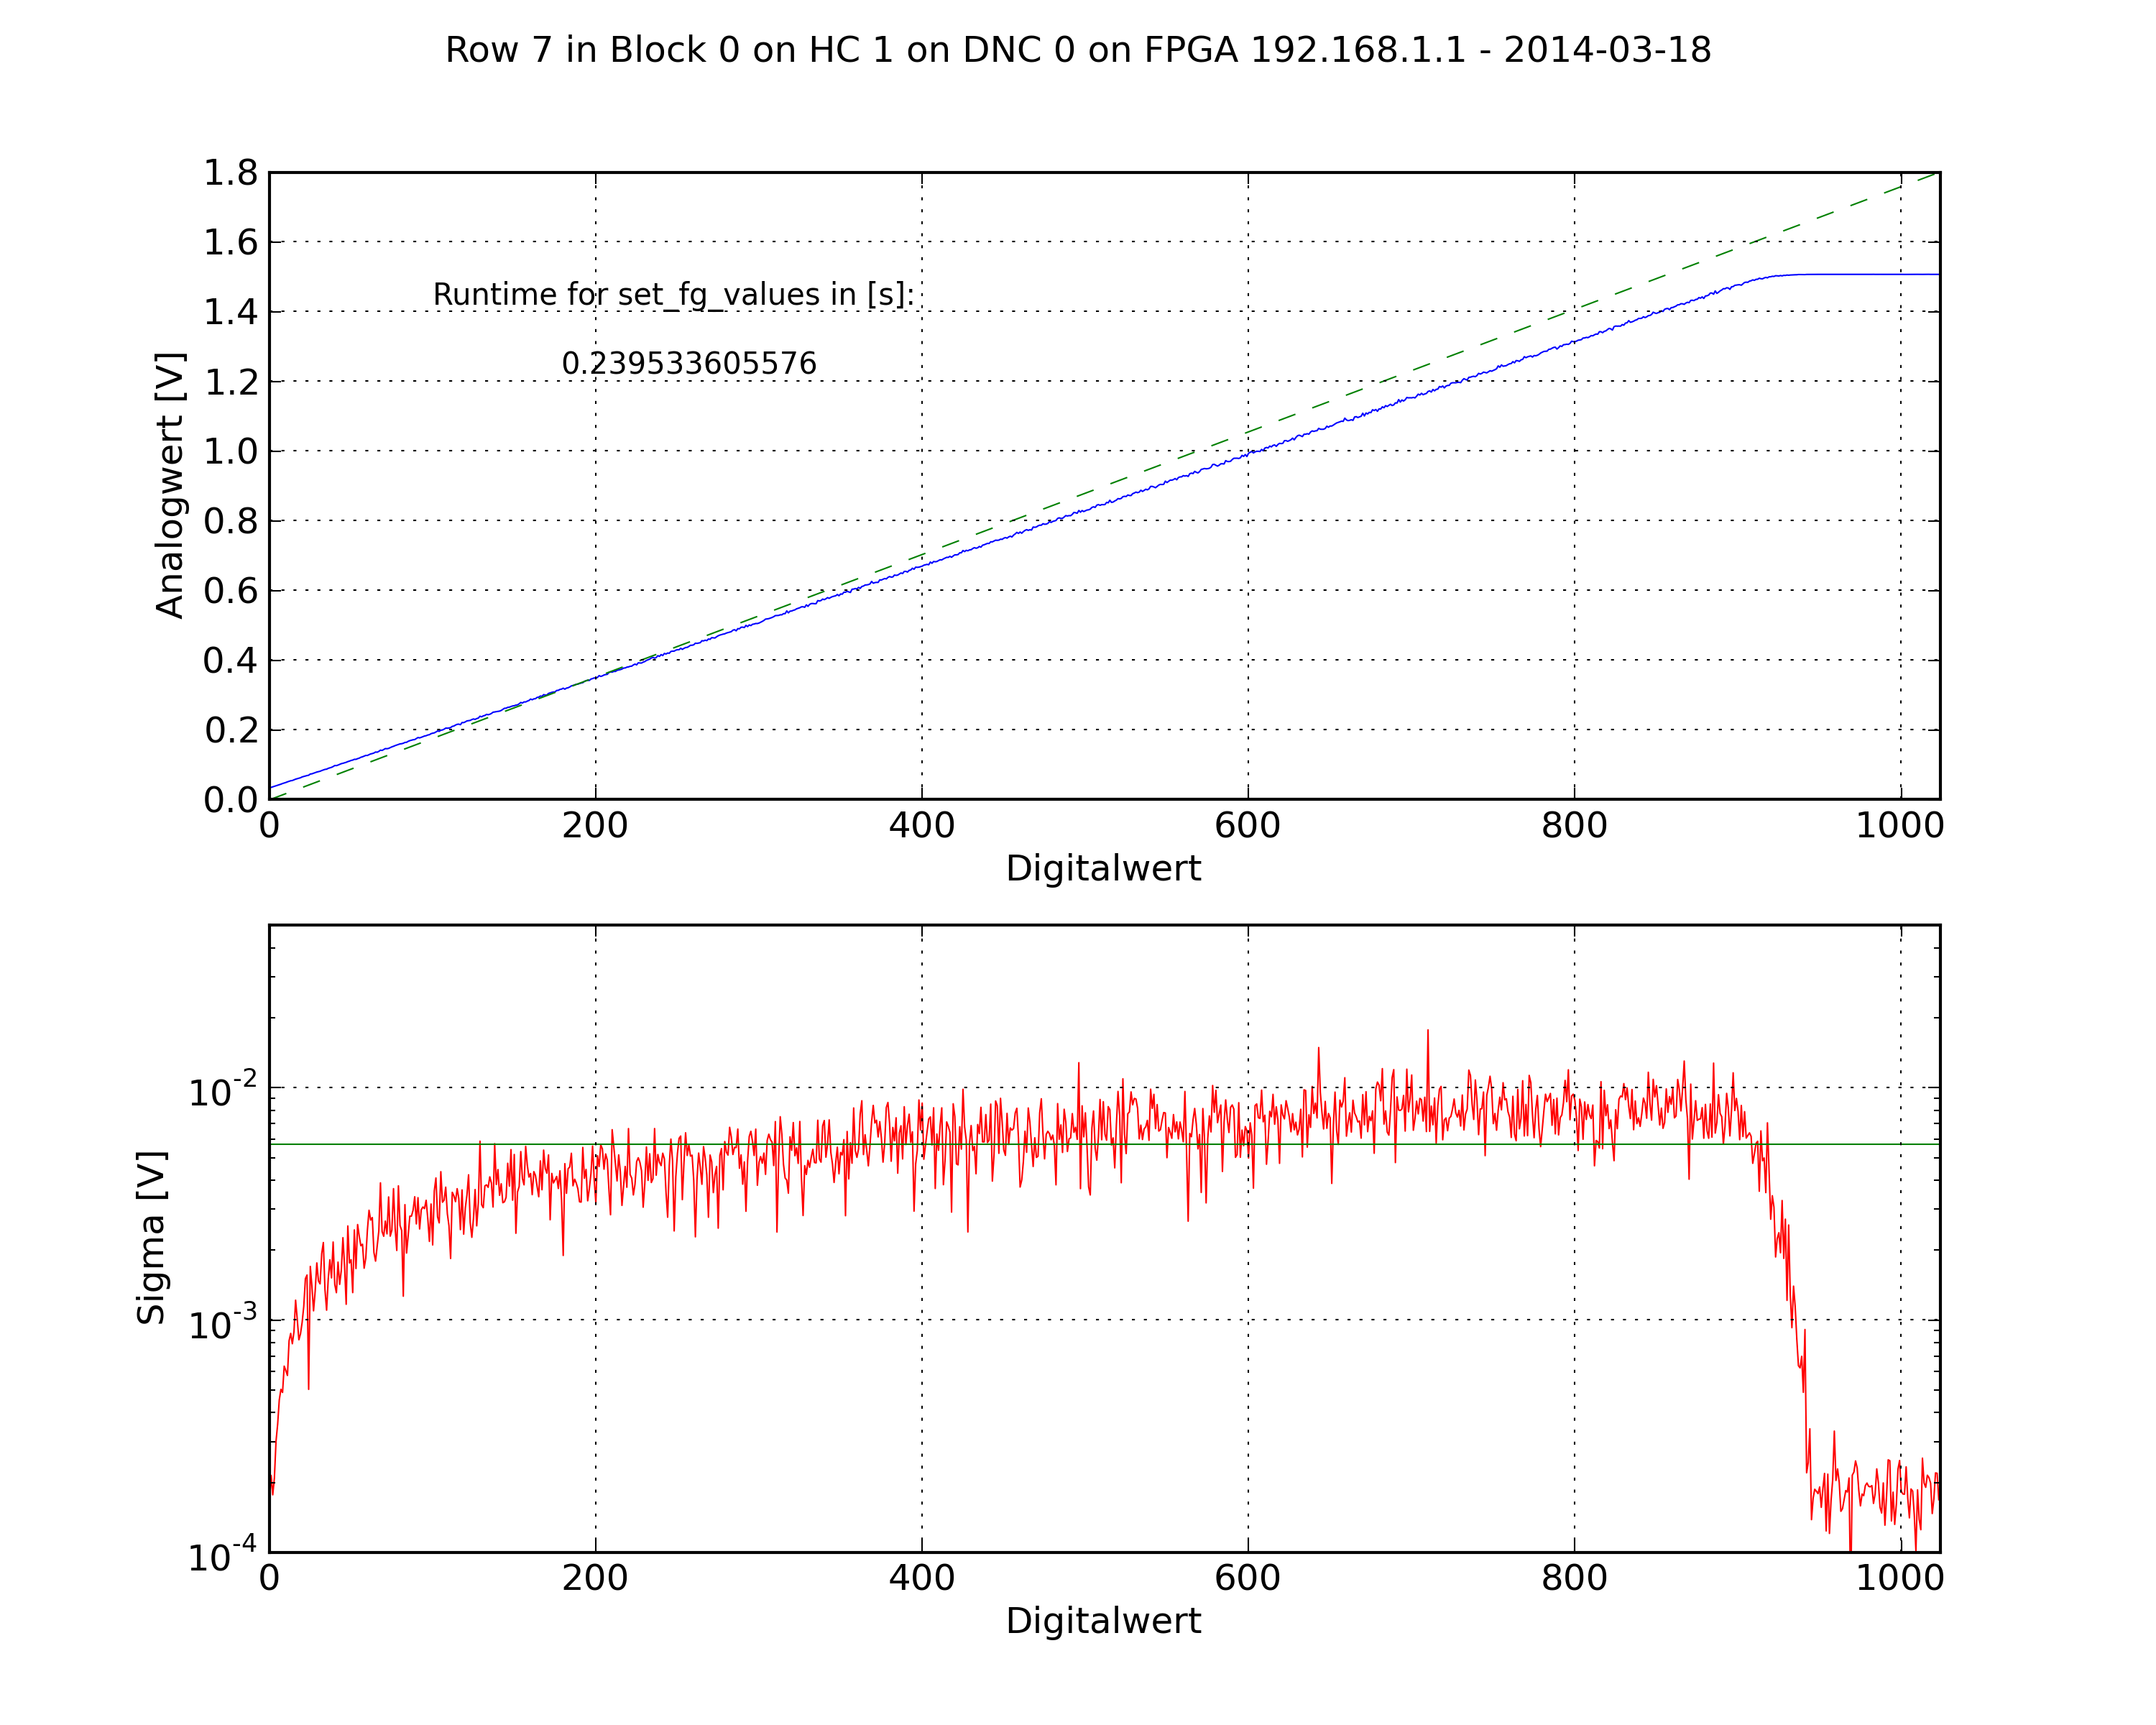
\includegraphics[scale=.28]{figures/single_row_random_progonerow_afterburn_current.png}
\caption{Voltage cells: 100 repeated runs of programming one single row to random values and reading out all cells of the row with the ADC board. The programming is done in two steps, once with default programming parameters and afterwards with short pulses.}
\label{fig:row_progrow_default_current}
\end{figure}

\section{Appendix}
Tabel \ref{tab:default_fg_values} shows the default programming parameters used for floating gate programming as of commit 1d15fd50.
\begin{table}
\begin{tabular}{l|l}
Parameter name & Register value\\
\hline
maxcycle & 255\\
readtime & 40\\
acceleratorstep & 9\\
voltagewritetime & 15\\
currentwritetime & 1\\
pulselength & 9\\
fg\_bias & 8\\
fg\_biasn & 5\\
groundvm & 0\\
calib & 0\\
\end{tabular}
\caption{Default floating gate operation parameters}
\label{tab:default_fg_values}
\end{table}

\begin{table}
\begin{tabular}{l|l}
Parameter name & Register value\\
\hline
maxcycle & 10\\
readtime & 63\\
acceleratorstep & 16\\
voltagewritetime & 5\\
currentwritetime & 20\\
pulselength & 1\\
fg\_bias & 8\\
fg\_biasn & 5\\
groundvm & 0\\
calib & 0\\
\end{tabular}
\caption{Floating gate operation parameters for higher precision with smaller programming pulses}
\label{tab:afterburn_fg_values}
\end{table}

\section{Tools}
This section describes the Python tools located in \texttt{tools/FG/}.
\begin{description}
	\item[FGTest.py] provides a test class for floating gate measurements that extends HWtest.
		It contains a rudimentary mapping of ADC boards to reticles and loads an appropriate ADC calibration for the ADC board in use.
		It also sets up the analog output of the floating gate chain and of the HICANN.
	\item[characterize\_FGs.py] writes a single row (as determined by self.row\_coord) to maximum DAC value and program it down with small single pulses of the floating gate controller.
		Measure new voltage afterwards and pickle the results to file FG\_characterize.txt
	\item[evaluate\_FG\_pulses.py]
		has to be used to evaluate the measurements done with characterize\_FGs.py.
		It plots the average voltage of the whole row (with standard deviation) after every programming pulse that has been applied.
		It also plots the average change in floating gate voltage as a function of the current floating gate voltage (given the current pulse width).
	\item[complete\_block\_repeat.py] programs a complete floating gate block to the same value for all cells in the block repeatedly and measures the output voltage for all cells.
		Writes results to \sloppy\texttt{./results/FG\%d\_HC\%d\_DNC\%d\_FPGA\%s\_\%d' \%(fg\_block\_num, self.HICANN, self.DNC, self.IP, target\_value\_volt) + ("" if reprogram else '\_norp')+'.pkl','wb')}.
	\item[plot\_fg\_block.py] plots the measurements done with complete\_block\_repeat.py.
		Gives a color map of the floating gate block with darker color representing a larger standard deviation with repeated measurements.
	\item[single\_row\_random\_values.py] writes random values to a single floating gate row, measures the resulting output voltage and plots mean value and standard deviation as a function of the target DAC value.
	\item[plot\_fg\_random\_row.py] contains the plotting function used to plot the data of single\_row\_random\_values.py.
		Plotted are the mean values for every digital target value in the upper plot and the standard deviation in the lower plot.
		The green line in these plots shows the average of the standard deviation for DAC values between 0 and 800.
\end{description}

%\begin{figure}
%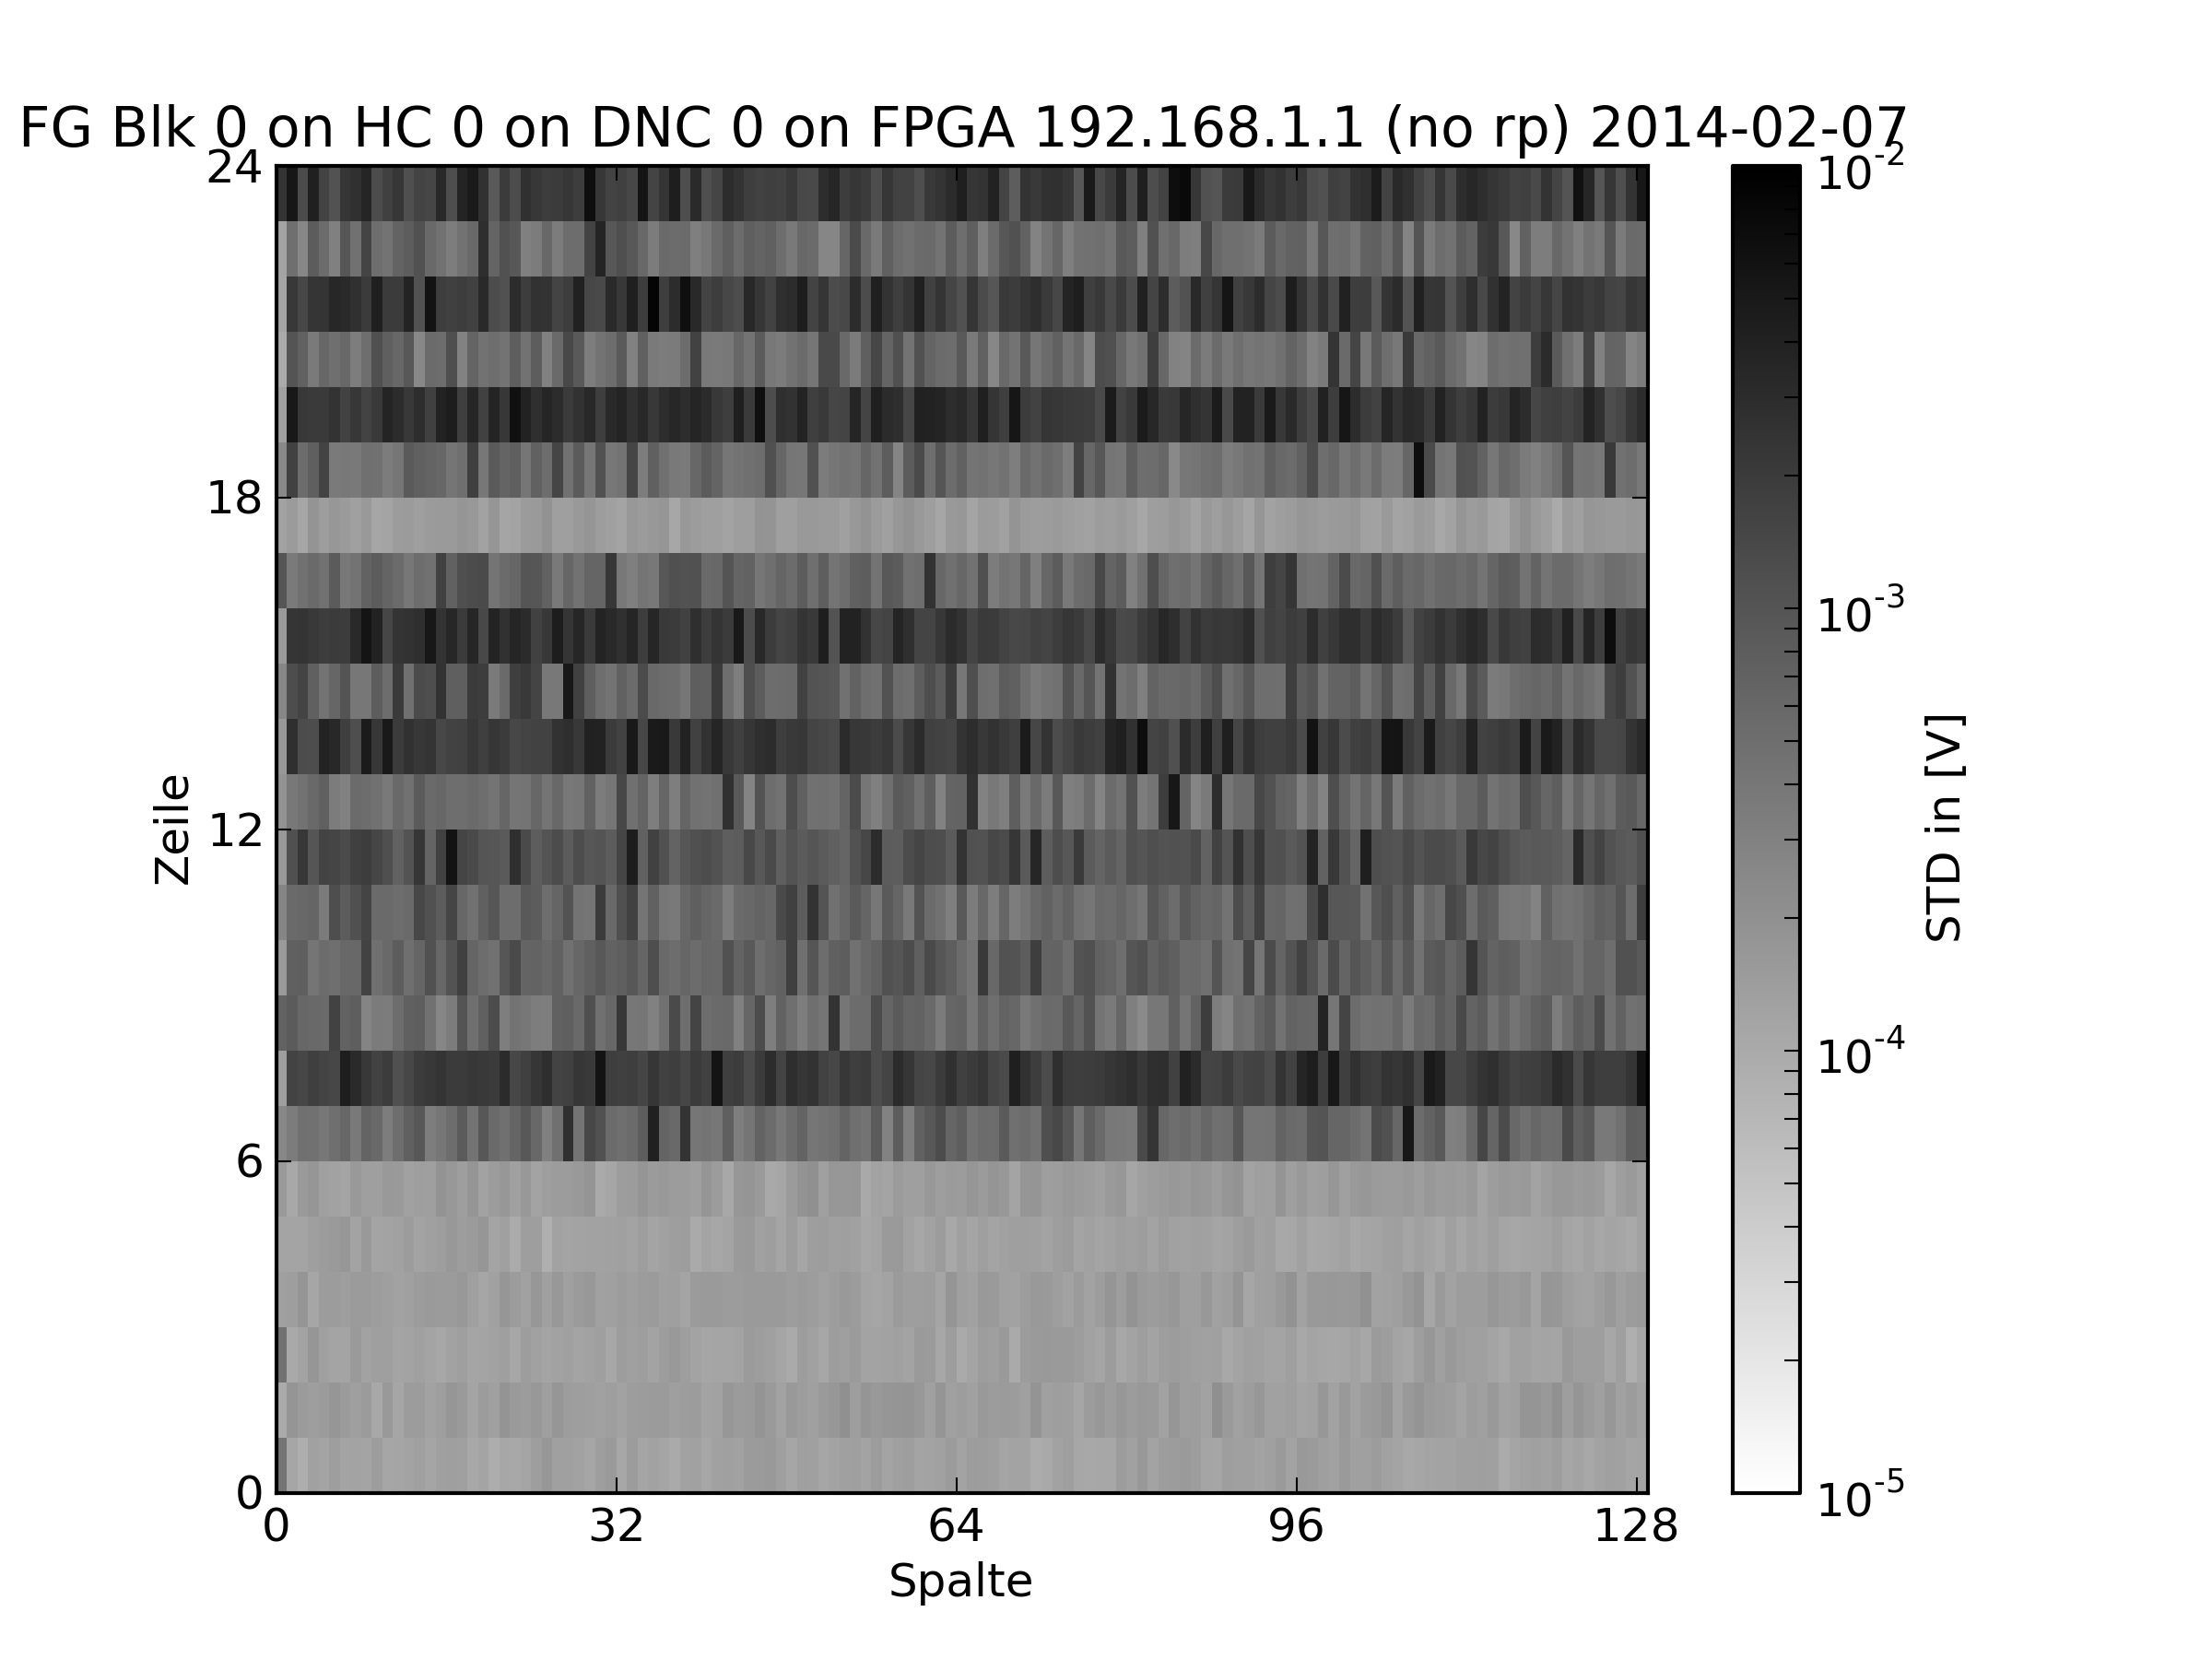
\includegraphics[scale=.34]{figures/program_block_defaults_measure_30times_5000samples.png}
%\end{figure}

\end{document}
